\section{Result}

\begin{figure}[H]
    \centering
    \begin{subfigure}[b]{0.99\textwidth} 
        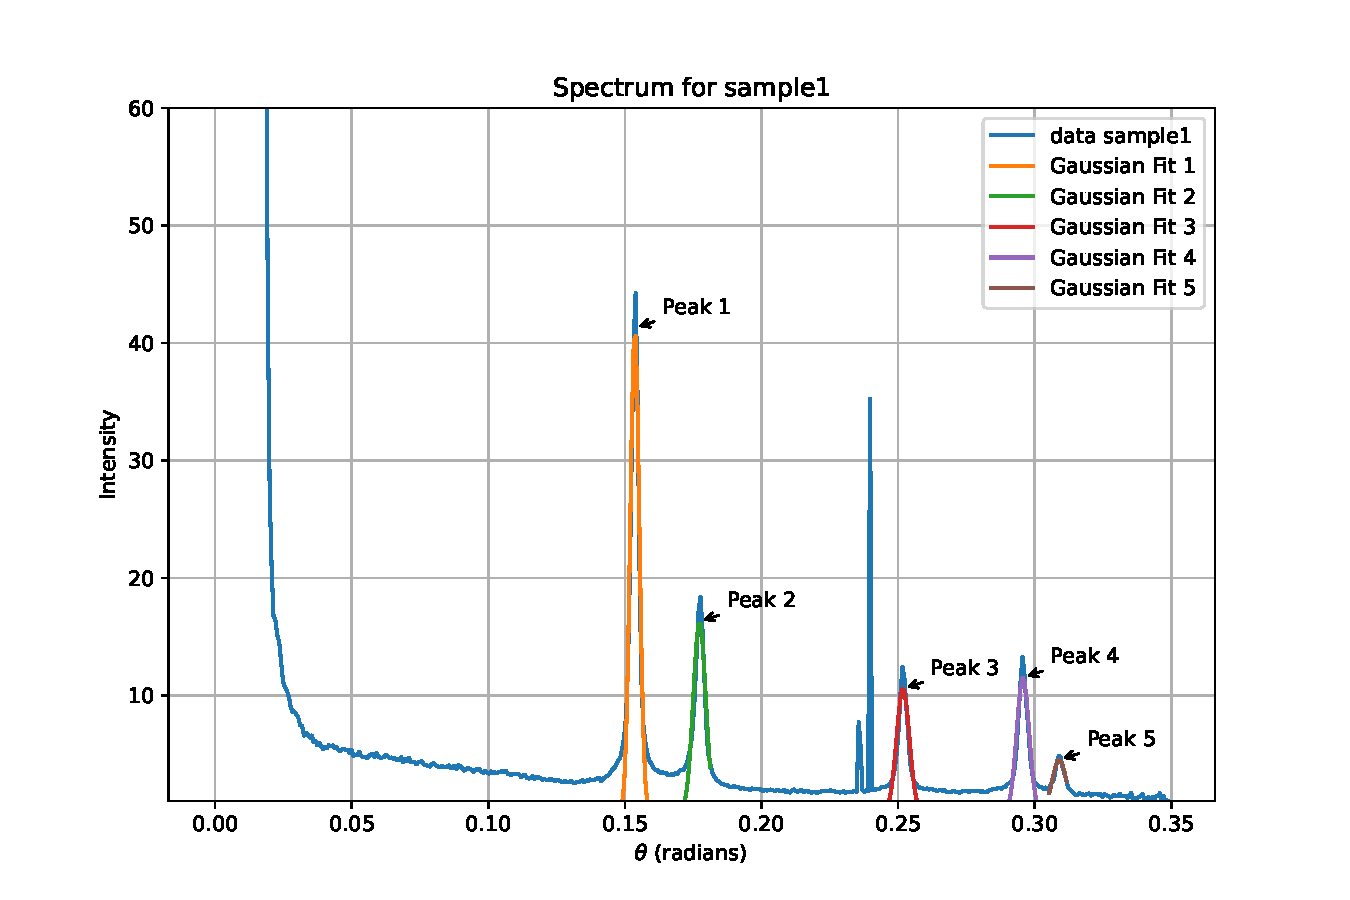
\includegraphics[width=\textwidth]{Figures/gaussian_sample1.pdf}
        \subcaption{This is the first subfigure.}
        \label{fig:subfigure1}
    \end{subfigure}
    \begin{subfigure}[b]{0.99\textwidth} 
        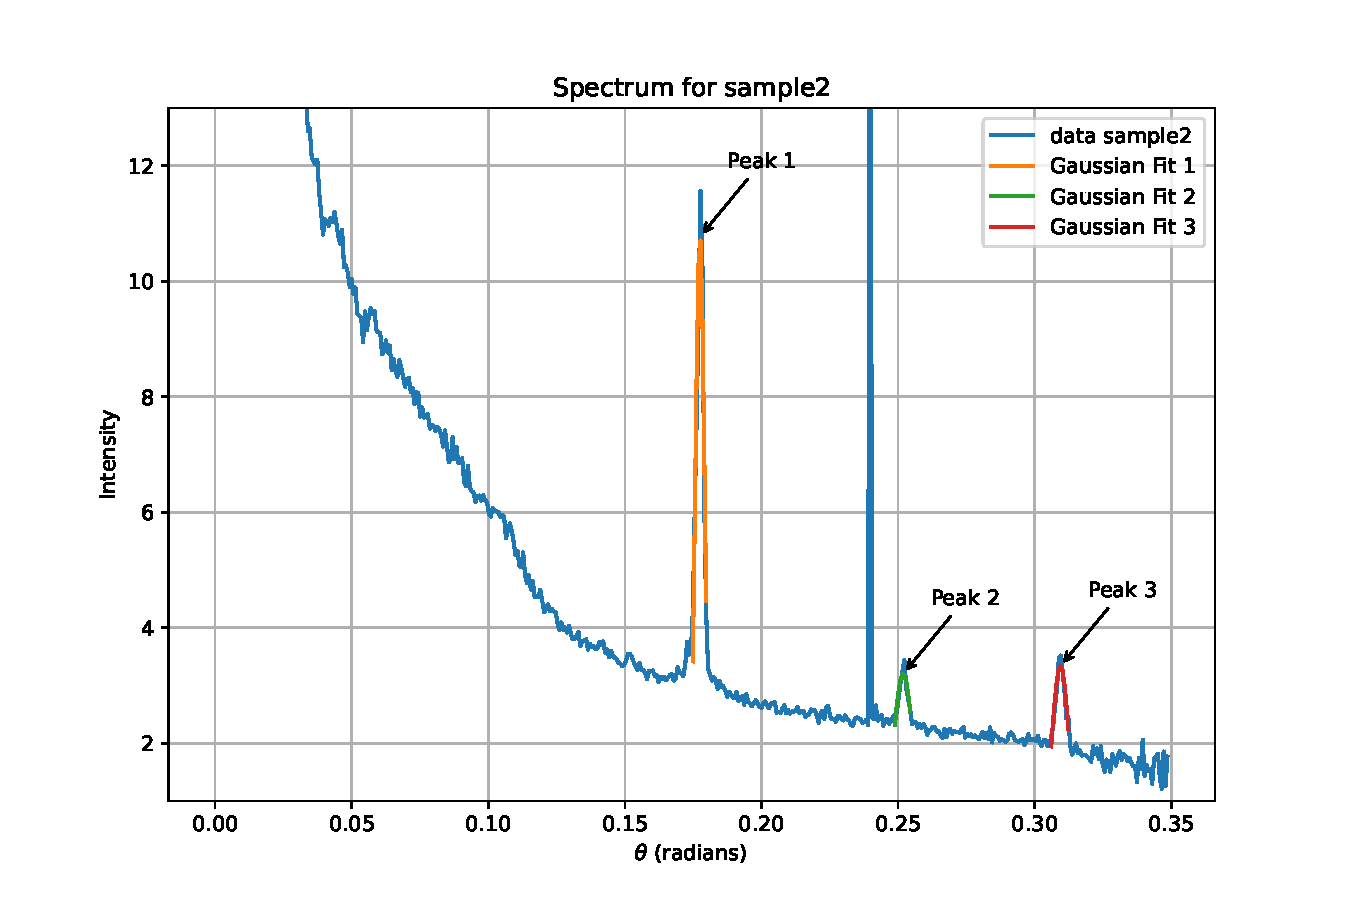
\includegraphics[width=\textwidth]{Figures/gaussian_sample2.pdf}
        \subcaption{This is the second subfigure.}
        \label{fig:subfigure2}
    \end{subfigure}
    \caption{This figure shows two subfigures with separate captions.}
    \label{fig:result_figure}
\end{figure}

\begin{table}[H]
    \centering
    \caption{Fitting results for Sample 1}
    \begin{tabular}{|c|c|c|c|}
    \hline
    Peak & Amplitude & Mean & FWHM \\
    \hline
    Peak 1 & \SI{41.29(2.15)}{units} & \SI{0.15362(0.00010)}{radians} & \SI{0.00388(0.00023)}{radians} \\
    \hline
    Peak 2 & \SI{16.28(1.14)}{units} & \SI{0.17731(0.00019)}{radians} & \SI{0.00535(0.00046)}{radians} \\
    \hline
    Peak 3 & \SI{10.57(0.71)}{units} & \SI{0.25180(0.00018)}{radians} & \SI{0.00550(0.00043)}{radians} \\
    \hline
    Peak 4 & \SI{11.53(0.66)}{units} & \SI{0.29569(0.00015)}{radians} & \SI{0.00530(0.00035)}{radians} \\
    \hline
    Peak 5 & \SI{4.51(0.19)}{units} & \SI{0.30900(0.00015)}{radians} & \SI{0.00616(0.00049)}{radians} \\
    \hline
    \end{tabular}
\end{table}

\begin{table}[H]
    \centering
    \caption{Fitting results for Sample 2}
    \begin{tabular}{|c|c|c|c|}
    \hline
    Peak & Amplitude & Mean & FWHM \\
    \hline
    Peak 1 & \SI{10.77(0.62)}{units} & \SI{0.17746(0.00012)}{radians} & \SI{0.00404(0.00034)}{radians} \\
    \hline
    Peak 2 & \SI{3.20(0.09)}{units} & \SI{0.25186(0.00017)}{radians} & \SI{0.00895(0.00092)}{radians} \\
    \hline
    Peak 3 & \SI{3.34(0.10)}{units} & \SI{0.30942(0.00014)}{radians} & \SI{0.00768(0.00056)}{radians} \\
    \hline
    \end{tabular}
\end{table}
